%=====================================================================
% PROJETO PREDIAL - LEITURA E INTERPRETACAO DA DOCUMENTACAO
%=====================================================================

\section{Leitura e interpretação de projetos elétricos}

\begin{frame}{Projeto elétrico é um conjunto coordenado de documentos}
\centering
\begin{tikzpicture}[
  b/.style={draw=corPrim,fill=corDef!7,rounded corners,minimum width=2.25cm,minimum height=0.75cm,align=center,font=\scriptsize},
  a/.style={-{Stealth},thick,corPrim}]
\node[b](pl)at(0,2.4){Plantas\\localização e rotas};
\node[b](dg)at(4.0,1.2){Diagramas\\lógica elétrica};
\node[b](qc)at(2.5,-1.8){Quadros e listas\\dados dos circuitos};
\node[b](mem)at(-2.5,-1.8){Memorial e cálculos\\critérios e resultados};
\node[b](det)at(-4.0,1.2){Detalhes\\como executar};
\node[draw=corAccent,fill=corAccent!12,rounded corners,minimum width=2.4cm,minimum height=0.85cm,align=center,font=\small\bfseries](obra)at(0,0.2){Instalação\\executável};
\foreach \x in {pl,dg,qc,mem,det}{\draw[a](\x)--(obra);}
\end{tikzpicture}
\vspace{2mm}
\begin{caixaAt}
Nenhum desenho deve ser lido isoladamente. A planta diz onde; o diagrama diz como; o quadro diz quanto; o memorial explica por quê; o detalhe mostra como executar.
\end{caixaAt}
\end{frame}

\begin{frame}{Antes de ler o desenho, leia a identificação}
\small
\begin{columns}[T,onlytextwidth]
\column{0.50\textwidth}
\begin{tikzpicture}[scale=0.78]
\draw[very thick] (0,0) rectangle (7.2,4.4);
\draw[thick] (4.45,0)--(4.45,1.45);
\draw[thick] (4.45,1.45)--(7.2,1.45);
\draw[thick] (5.85,0)--(5.85,1.45);
\node[font=\scriptsize\bfseries] at (5.83,1.15){PROJETO ELÉTRICO};
\node[font=\tiny,align=left,anchor=west] at (4.62,0.72){Prancha: PE-03\\Pavimento: térreo};
\node[font=\tiny,align=left,anchor=west] at (6.0,0.72){Rev.: 04\\Esc.: 1:50};
\node[font=\tiny,anchor=west] at (0.25,4.05){PLANTA DE ILUMINAÇÃO};
\draw[corAccent,thick,dashed] (4.55,0.15) rectangle (7.05,1.3);
\node[font=\tiny,corAccent] at (5.8,-0.35){carimbo e revisão};
\end{tikzpicture}
\column{0.48\textwidth}
\begin{enumerate}
\item título e finalidade da prancha;
\item edifício, pavimento e área;
\item código, escala e unidade;
\item revisão e data de emissão;
\item responsável e status do documento;
\item notas gerais e referências cruzadas;
\item legenda aplicável àquela prancha.
\end{enumerate}
\end{columns}
\begin{caixaAt}
Não executar prancha superada, sem revisão ou emitida apenas para estudo/coordenação.
\end{caixaAt}
\end{frame}

\begin{frame}{Linhas, símbolos e textos formam uma linguagem}
\small
\begin{tabularx}{\textwidth}{>{\bfseries}p{2.5cm}p{3.0cm}X}
\toprule
Elemento & Exemplo gráfico & O que interpretar \\
\midrule
Linha contínua & \tikz\draw[corPrim,thick](0,0)--(2.2,0); & ligação ou limite físico conforme a legenda \\
Linha tracejada & \tikz\draw[corAccent,thick,dashed](0,0)--(2.2,0); & comando, circuito, rota oculta ou referência \\
Seta & \tikz\draw[-{Stealth},corPrim,thick](0,0)--(2.2,0); & sentido funcional, fluxo ou continuação \\
Nó preenchido & \tikz\fill[corPrim](0,0)circle(2.4pt); & conexão elétrica efetiva \\
Cruzamento sem nó & \tikz{\draw[corPrim](0,-0.25)--(0,0.25);\draw[corPrim](-0.4,0)--(0.4,0);} & linhas cruzam sem conexão, salvo convenção diferente \\
Etiqueta C7 & \fbox{C7} & circuito que remete ao quadro de cargas \\
Referência 4/PE-08 & \fbox{4/PE-08} & detalhe 4 na prancha PE-08 \\
\bottomrule
\end{tabularx}
\begin{caixaObs}
Convenções variam. A legenda e as notas do projeto prevalecem sobre hábitos de leitura.
\end{caixaObs}
\end{frame}

\begin{frame}{Símbolo só tem significado completo com atributos}
\small
\begin{columns}[T,onlytextwidth]
\column{0.50\textwidth}
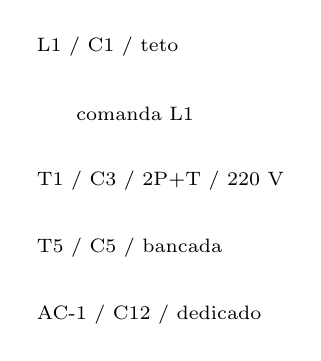
\begin{tikzpicture}[every node/.style={font=\scriptsize}]
\SimLuz{0.4}{3.9}\node[anchor=west]at(1.0,3.9){L1 / C1 / teto};
\SimInterruptor{0.4}{3.05}{S1}\node[anchor=west]at(1.5,3.05){comanda L1};
\SimTUG{0.4}{2.2}\node[anchor=west]at(1.0,2.2){T1 / C3 / 2P+T / 220 V};
\SimTUGM{0.4}{1.35}\node[anchor=west]at(1.0,1.35){T5 / C5 / bancada};
\SimTUE{0.4}{0.5}{E}\node[anchor=west]at(1.0,0.5){AC-1 / C12 / dedicado};
\end{tikzpicture}
\column{0.48\textwidth}
Para cada ponto, procurar:
\begin{itemize}
\item identificador único;
\item circuito e fase;
\item tensão e número de polos;
\item altura/cota de montagem;
\item potência ou equipamento;
\item comando associado;
\item nota ou detalhe construtivo.
\end{itemize}
\end{columns}
\begin{caixaAt}
Um círculo na planta não diz sozinho qual cabo, proteção, altura ou ligação usar. Esses dados vêm da etiqueta e dos documentos associados.
\end{caixaAt}
\end{frame}

\begin{frame}{Da arquitetura à planta elétrica}
\centering
\begin{tikzpicture}[scale=0.78]
\begin{scope}[xshift=-7.0cm]
\draw[very thick](0,0)rectangle(5.8,4.2);
\draw[thick](0,1.5)--(5.8,1.5);\draw[thick](3.7,1.5)--(3.7,4.2);
\node[font=\scriptsize\bfseries]at(1.85,3.7){SALA};
\node[font=\scriptsize\bfseries]at(4.75,3.7){COZINHA};
\node[font=\scriptsize\bfseries]at(2.9,0.75){QUARTO};
\draw[white,line width=5pt](1.0,1.5)--(1.9,1.5);\draw(1.0,1.5)--(1.9,2.4);
\node[font=\scriptsize]at(2.9,-0.55){planta arquitetônica};
\end{scope}
\draw[-{Stealth},very thick,corAccent](-0.8,2.1)--(0.8,2.1);
\begin{scope}[xshift=1.6cm]
\draw[very thick](0,0)rectangle(5.8,4.2);
\draw[thick](0,1.5)--(5.8,1.5);\draw[thick](3.7,1.5)--(3.7,4.2);
\node[font=\scriptsize\bfseries]at(1.85,3.7){SALA};
\node[font=\scriptsize\bfseries]at(4.75,3.7){COZINHA};
\node[font=\scriptsize\bfseries]at(2.9,0.75){QUARTO};
\draw[white,line width=5pt](1.0,1.5)--(1.9,1.5);\draw(1.0,1.5)--(1.9,2.4);
\SimQD{0.4}{2.1}{QD}
\SimLuz{1.9}{2.8}\SimLuz{4.75}{2.8}\SimLuz{2.9}{0.65}
\SimInterruptor{1.05}{1.75}{S1}
\foreach \x/\y in {0.25/2.3,3.45/2.3,4.0/1.8,5.55/2.2,0.25/0.3,5.55/0.3}{\SimTUG{\x}{\y}}
\draw[corAccent,dashed,thick](0.4,2.1)--(1.9,2.8)--(4.75,2.8);
\draw[corPrim,dashed,thick](0.4,2.1)--(0.25,2.3)--(3.45,2.3);
\node[font=\scriptsize]at(2.9,-0.55){planta elétrica coordenada};
\end{scope}
\end{tikzpicture}
\begin{caixaObs}
Portas definem comandos; mobiliário define tomadas; paredes e vigas limitam rotas; uso do ambiente define cargas e proteção.
\end{caixaObs}
\end{frame}

\begin{frame}{Siga um circuito da origem até cada ponto}
\centering
\begin{tikzpicture}[scale=0.82]
\draw[very thick](0,0)rectangle(11.8,5.4);
\draw[thick](4.2,0)--(4.2,5.4);\draw[thick](8.0,0)--(8.0,5.4);
\node[font=\scriptsize\bfseries]at(2.1,5.0){SALA};
\node[font=\scriptsize\bfseries]at(6.1,5.0){COZINHA};
\node[font=\scriptsize\bfseries]at(9.9,5.0){SERVIÇO};
\SimQD{0.55}{2.7}{QD1}
\SimLuz{2.1}{3.0}\SimLuz{6.1}{3.0}\SimLuz{9.9}{3.0}
\SimInterruptor{1.0}{0.45}{S1}\SimInterruptor{5.0}{0.45}{S2}\SimInterruptor{8.9}{0.45}{S3}
\draw[corAccent,line width=2.2pt,-{Stealth}](0.85,2.7)--(2.1,3.0)--(6.1,3.0)--(9.9,3.0);
\node[font=\scriptsize\bfseries,fill=white,corAccent]at(5.8,3.35){C1};
\draw[corNorma,dashed,thick](1.0,0.45)--(2.1,3.0);
\draw[corNorma,dashed,thick](5.0,0.45)--(6.1,3.0);
\draw[corNorma,dashed,thick](8.9,0.45)--(9.9,3.0);
\end{tikzpicture}
\vspace{1mm}
\begin{enumerate}
\item localizar C1 no quadro de cargas;
\item identificar origem, fase, neutro e PE no QD1;
\item seguir a rota e contar pontos/caixas;
\item conferir comandos S1--S3 e luminárias associadas;
\item cruzar seção, proteção, comprimento e queda.
\end{enumerate}
\end{frame}

\begin{frame}{A mesma instalação em quatro representações}
\scriptsize
\begin{columns}[T,onlytextwidth]
\column{0.24\textwidth}
\centering\textbf{Planta}\par\vspace{1mm}
\begin{tikzpicture}[scale=0.52]
\draw(0,0)rectangle(4,3);\SimQD{0.35}{1.5}{QD}\SimLuz{2.6}{1.7}\SimInterruptor{1.0}{0.35}{S}
\draw[corAccent,dashed,thick](0.65,1.5)--(2.6,1.7);\draw[corNorma,dashed](1.0,0.35)--(2.6,1.7);
\end{tikzpicture}
\column{0.24\textwidth}
\centering\textbf{Unifilar}\par\vspace{1mm}
\begin{circuitikz}[scale=0.58,transform shape]
\draw (0,2.6) node[left]{QD} to[short,o-] (0.8,2.6) to[ospst=$Q_1$] (2.0,2.6) to[lamp,l=$L_1$] (2.0,0) node[ground]{};
\end{circuitikz}
\column{0.24\textwidth}
\centering\textbf{Multifilar}\par\vspace{1mm}
\begin{circuitikz}[scale=0.50,transform shape]
\draw[corPrim] (0,3)--(3.4,3)node[right]{F};
\draw[corDef] (0,0)--(3.4,0)node[right]{N};
\draw[corNorma] (0,-0.55)--(3.4,-0.55)node[right]{PE};
\draw (0.65,3)to[ospst=$S_1$](2.25,3)to[lamp,l=$L_1$](2.25,0);
\end{circuitikz}
\column{0.24\textwidth}
\centering\textbf{Ligação física}\par\vspace{1mm}
\begin{tikzpicture}[scale=0.53]
\node[draw,minimum width=1.1cm,minimum height=1.0cm](s)at(0,0){S1};
\node[draw,circle,minimum size=0.9cm](l)at(2.8,2.3){L1};
\draw[corPrim,thick](s.west)--(-0.7,0)node[left]{F};
\draw[corAccent,thick](s.east)--(l.west);
\draw[corDef,thick](-0.7,2.7)node[left]{N}--(l.north);
\draw[corNorma,thick](-0.7,2.25)node[left]{PE}--(l.south);
\end{tikzpicture}
\end{columns}
\vspace{3mm}
\begin{caixaObs}
Planta localiza; unifilar resume; multifilar explicita condutores; ligação física mostra bornes e passagem real.
\end{caixaObs}
\end{frame}

\begin{frame}[shrink=4]{Como ler um diagrama unifilar}
\centering
\begin{tikzpicture}[
  b/.style={draw=corPrim,fill=corDef!7,rounded corners,minimum width=2.0cm,minimum height=0.7cm,align=center,font=\scriptsize}]
\node[b](orig)at(0,4.2){Rede 380/220 V};
\node[b](dg)at(0,3.1){DG 3P 63 A};
\node[b](dps)at(0,2.0){DPS + DR geral\\quando aplicável};
\node[b](qd)at(0,0.9){Barramentos\\F / N / PE};
\node[b](c1)at(-4.0,-0.8){C1 iluminação\\10 A / 1,5 mm$^2$};
\node[b](c2)at(-1.35,-0.8){C2 TUG\\16 A / 2,5 mm$^2$};
\node[b](c3)at(1.35,-0.8){C3 chuveiro\\32 A / 6 mm$^2$};
\node[b](c4)at(4.0,-0.8){C4 SAVE\\40 A / 10 mm$^2$};
\draw[-{Stealth},thick,corPrim](orig)--(dg)--(dps)--(qd);
\foreach \x in {c1,c2,c3,c4}{\draw[-{Stealth},thick](qd)--(\x);}
\end{tikzpicture}
\begin{caixaNorma}
Leia de cima para baixo: origem e tensão, seccionamento, proteção contra surtos/choque, barramentos, circuitos terminais e dados de cada saída.
\end{caixaNorma}
\end{frame}

\begin{frame}[shrink=4]{Como ler um diagrama multifilar}
\centering
\begin{circuitikz}[scale=0.92,transform shape]
\draw[corPrim,thick] (-5,2.4)--(5.2,2.4) node[right]{F};
\draw[corDef,thick] (-5,-0.9)--(5.2,-0.9) node[right]{N};
\draw[corNorma,thick] (-5,-1.55)--(5.2,-1.55) node[right]{PE};
\draw[corPrim] (-4.2,2.4) to[ospst,l=$Q_1$] (-2.3,2.4) to[ospst,l=$S_1$] (-0.3,2.4) to[lamp,l=$L_1$] (-0.3,-0.9);
\draw[corNorma,thick] (-0.3,-1.55)--(-0.3,-1.25);
\draw[corPrim] (1.0,2.4) to[ospst,l=$Q_2$] (2.9,2.4)--(2.9,0.35);
\draw[corDef] (2.9,0.35)--(2.9,-0.9);
\draw[corNorma] (3.45,0.35)--(3.45,-1.55);
\draw (2.55,0.35) rectangle (3.8,-0.35);
\node[font=\scriptsize] at (3.18,0){T1 2P+T};
\end{circuitikz}
\vspace{1mm}
\begin{columns}[T,onlytextwidth]
\column{0.49\textwidth}
\begin{itemize}
\item cada condutor é desenhado separadamente;
\item nós mostram conexões elétricas;
\item contatos aparecem na condição de repouso;
\end{itemize}
\column{0.49\textwidth}
\begin{itemize}
\item cores no desenho são didáticas, não substituem etiquetas;
\item acompanhar fase, neutro e PE até a carga;
\item conferir polos interrompidos e protegidos.
\end{itemize}
\end{columns}
\end{frame}

\begin{frame}{Funcional e ligação física respondem perguntas diferentes}
\small
\begin{columns}[T,onlytextwidth]
\column{0.49\textwidth}
\centering\textbf{Diagrama funcional}\par\vspace{1mm}
\begin{circuitikz}[scale=0.76,transform shape]
\draw (0,3)node[left]{F}to[ospst,l=$S_1$](2,3)to[lamp,l=$L_1$](2,0)node[left]{N};
\end{circuitikz}
\begin{itemize}
\item mostra a lógica de funcionamento;
\item simplifica caixas e percurso;
\item facilita análise de estados.
\end{itemize}
\column{0.49\textwidth}
\centering\textbf{Esquema de ligação}\par\vspace{1mm}
\begin{tikzpicture}[scale=0.7]
\node[draw,minimum width=1.3cm,minimum height=1.1cm](cx)at(0,1.4){4x2};
\node[draw,circle,minimum size=1.0cm](l)at(3.8,3.1){L1};
\draw[corPrim,thick](-1.3,1.4)node[left]{F}--(cx.west);
\draw[corAccent,thick](cx.east)--(l.west);
\draw[corDef,thick](-1.3,3.5)node[left]{N}--(l.north);
\draw[corNorma,thick](-1.3,2.9)node[left]{PE}--(l.south);
\end{tikzpicture}
\begin{itemize}
\item mostra caixas, bornes e condutores;
\item orienta passagem e terminação;
\item precisa corresponder ao funcional.
\end{itemize}
\end{columns}
\end{frame}

\begin{frame}{Layout do quadro não substitui o unifilar}
\small
\begin{columns}[T,onlytextwidth]
\column{0.49\textwidth}
\centering\textbf{Layout físico}\par\vspace{1mm}
\begin{tikzpicture}[scale=0.72]
\draw[very thick](0,0)rectangle(6.4,4.8);
\draw[thick](0.35,3.55)--(6.05,3.55);\draw[thick](0.35,1.75)--(6.05,1.75);
\foreach \x/\t in {0.75/DG,1.75/DPS,2.75/DR,3.75/C1,4.55/C2,5.35/C3}{
  \draw[fill=corDef!7,draw=corPrim](\x-0.35,2.2)rectangle(\x+0.35,3.3);
  \node[font=\tiny]at(\x,2.75){\t};}
\draw[corDef,thick](0.7,0.7)--(5.7,0.7)node[right,font=\tiny]{N};
\draw[corNorma,thick](0.7,0.35)--(5.7,0.35)node[right,font=\tiny]{PE};
\end{tikzpicture}
\column{0.49\textwidth}
\centering\textbf{Unifilar associado}\par\vspace{1mm}
\begin{tikzpicture}[
  b/.style={draw=corPrim,fill=corDef!7,minimum width=1.45cm,minimum height=0.55cm,font=\tiny,align=center}]
\node[b](dg)at(0,4.0){DG};\node[b](dps)at(0,3.1){DPS};\node[b](dr)at(0,2.2){DR};
\node[b](c1)at(-2.2,0.8){C1};\node[b](c2)at(0,0.8){C2};\node[b](c3)at(2.2,0.8){C3};
\draw[-{Stealth},thick,corPrim](dg)--(dps)--(dr);
\foreach \x in {c1,c2,c3}{\draw[-{Stealth},thick](dr)--(\x);}
\end{tikzpicture}
\end{columns}
\begin{caixaAt}
Layout indica posição e montagem. Unifilar indica relação elétrica. Ambos precisam usar os mesmos códigos e dispositivos.
\end{caixaAt}
\end{frame}

\begin{frame}[shrink=4]{Quadro de cargas conecta planta, diagrama e cálculo}
\scriptsize
\begin{tabularx}{\textwidth}{c X c c c c c c}
\toprule
C & Descrição & Pontos & Fase & $I_b$ & Cabo & DJ/DR & Prancha \\
\midrule
C1 & iluminação sala/cozinha & 7 & A & 4,8 A & 1,5 mm$^2$ & 10 A / RCBO & PE-02 \\
C2 & iluminação íntima & 6 & B & 6,4 A & 1,5 mm$^2$ & 10 A / RCBO & PE-02 \\
C3 & TUG sala/quartos & 17 & C & 7,7 A & 2,5 mm$^2$ & 16 A / DR & PE-03 \\
C5 & TUG cozinha & 6 & B & 9,5 A & 2,5 mm$^2$ & 16 A / DR & PE-03 \\
C9 & chuveiro social & 1 & A & 25,0 A & 6 mm$^2$ & 32 A / DR & PE-04 \\
\bottomrule
\end{tabularx}
\vspace{2mm}
\begin{caixaNorma}
Ao localizar C9 na planta, o quadro informa fase, corrente, seção e proteção; o unifilar mostra origem e dispositivo; o detalhe PE-04 mostra a ligação e a terminação.
\end{caixaNorma}
\end{frame}

\begin{frame}{Diagrama vertical: leia por pavimento e por sistema}
\centering
\begin{tikzpicture}[scale=0.8]
\draw[very thick](0,0)rectangle(10.5,5.2);
\foreach \y/\p in {0.8/Térreo,2.2/1º pav.,3.6/2º pav.,4.8/Cobertura}{
  \draw[black!35](0,\y)--(10.5,\y);\node[font=\tiny,anchor=east]at(-0.15,\y){\p};}
\draw[corPrim,line width=3pt](3.3,0.4)--(3.3,4.95);
\draw[corNorma,line width=3pt](6.7,0.4)--(6.7,4.95);
\node[font=\scriptsize\bfseries,corPrim]at(3.3,5.55){prumada de energia};
\node[font=\scriptsize\bfseries,corNorma]at(6.7,5.55){BEP / PE};
\foreach \y/\q [count=\i] in {0.8/QD-T,2.2/QD-1,3.6/QD-2}{
  \node[draw=corPrim,fill=corDef!7,minimum width=1.3cm,minimum height=0.48cm,font=\tiny](q\i)at(1.65,\y){\q};
  \draw[-{Stealth},thick,corPrim](3.3,\y)--(q\i);
  \draw[thick,corNorma](q\i)--(6.7,\y);}
\node[draw=corAccent,fill=corAccent!10,font=\tiny,align=center]at(8.7,4.35){SPDA\\cobertura};
\draw[thick,corNorma](8.7,4.0)--(6.7,3.6);
\end{tikzpicture}
\begin{caixaObs}
O vertical mostra origem, prumadas, quadros por pavimento, seções, proteção e equipotencialização. Ele não mostra a posição de cada tomada.
\end{caixaObs}
\end{frame}

\begin{frame}{Esquema de aterramento muda a leitura da proteção}
\scriptsize
\begin{columns}[T,onlytextwidth]
\column{0.32\textwidth}
\centering\textbf{TN-S}\par
\begin{tikzpicture}[scale=0.55]
\node[draw](f)at(0,2.8){Fonte};\node[draw](c)at(0,0){Carga};
\draw[corPrim,thick](f)--(-0.7,1.4)--(c);
\draw[corDef,thick](f)--(0,1.4)--(c);
\draw[corNorma,thick](f)--(0.7,1.4)--(c);
\node[font=\tiny]at(-0.9,1.4){F};\node[font=\tiny]at(-0.15,1.4){N};\node[font=\tiny]at(0.9,1.4){PE};
\end{tikzpicture}
\column{0.32\textwidth}
\centering\textbf{TT}\par
\begin{tikzpicture}[scale=0.55]
\node[draw](f)at(0,2.8){Fonte};\node[draw](c)at(0,0){Carga};
\draw[corPrim,thick](f)--(-0.55,1.4)--(c);
\draw[corDef,thick](f)--(0.15,1.4)--(c);
\draw[corNorma,thick](c.south)--(0,-0.8)node[ground]{};
\draw[corNorma,thick](f.south east)--(1.2,2.0)node[ground]{};
\node[draw=corAt,fill=corAt!7,font=\tiny]at(1.25,0.5){DR};
\end{tikzpicture}
\column{0.32\textwidth}
\centering\textbf{IT}\par
\begin{tikzpicture}[scale=0.55]
\node[draw](f)at(0,2.8){Fonte};\node[draw](c)at(0,0){Carga};
\draw[corPrim,thick](f)--(-0.45,1.4)--(c);
\draw[corDef,thick](f)--(0.25,1.4)--(c);
\draw[corNorma,thick](c.south)--(0,-0.8)node[ground]{};
\draw[dashed,corNorma](f.south east)--(1.2,2.0)node[ground]{};
\node[font=\tiny]at(1.0,1.25){isolado/impedância};
\end{tikzpicture}
\end{columns}
\begin{caixaAt}
Não interpretar proteção contra choque sem identificar o esquema. Caminho da falta, DR, equipotencialização e desligamento dependem dele.
\end{caixaAt}
\end{frame}

\begin{frame}{Referências cruzadas evitam repetir desenho}
\small
\begin{columns}[T,onlytextwidth]
\column{0.48\textwidth}
\begin{tikzpicture}[scale=0.76]
\draw[very thick](0,0)rectangle(6.5,4.5);
\node[draw=corAccent,circle,minimum size=0.75cm,font=\scriptsize\bfseries](d)at(3.2,2.4){4};
\draw[corAccent,thick](d)--(5.2,3.6);
\node[draw=corPrim,fill=corDef!7,font=\scriptsize]at(5.2,3.9){4/PE-08};
\node[font=\scriptsize]at(3.25,-0.55){planta PE-03};
\end{tikzpicture}
\column{0.50\textwidth}
\begin{tikzpicture}[scale=0.76]
\draw[very thick](0,0)rectangle(6.5,4.5);
\node[font=\scriptsize\bfseries]at(3.25,4.1){DETALHE 4 — PE-08};
\node[draw=corPrim,minimum width=2.1cm,minimum height=0.9cm]at(3.25,2.5){caixa / ligação};
\draw[corPrim,thick](3.25,2.05)--(3.25,0.7);
\node[font=\scriptsize]at(3.25,-0.55){prancha de detalhes};
\end{tikzpicture}
\end{columns}
\begin{caixaObs}
Leia o número do detalhe e a prancha de destino. Depois retorne à planta e confira se a condição detalhada é a mesma do ponto executado.
\end{caixaObs}
\end{frame}

\begin{frame}{Interprete por circuito, não apenas por prancha}
\small
\begin{enumerate}
\item escolha um circuito no quadro de cargas;
\item localize proteção e barramentos no unifilar;
\item encontre todos os pontos identificados na planta;
\item siga a rota e anote caixas, derivações e comprimentos;
\item abra os detalhes e esquemas de ligação associados;
\item confira seção, número de condutores e identificação;
\item verifique memorial, queda, DR, DPS e notas especiais;
\item confirme que a lista de materiais contempla o circuito.
\end{enumerate}
\begin{caixaProjeto}
Ao final, o aluno deve conseguir narrar o circuito: de onde vem, por onde passa, como é protegido, como funciona, onde termina e como será testado.
\end{caixaProjeto}
\end{frame}

\begin{frame}{Inconsistências entre planta, quadro e unifilar}
\scriptsize
\begin{tabularx}{\textwidth}{>{\bfseries}p{3.2cm}X}
\toprule
Conflito & Como perceber \\
\midrule
Circuito existe na planta, mas não no quadro & conferir todos os códigos Cx \\
Disjuntor e cabo divergem do unifilar & cruzar corrente, seção e proteção \\
Tomada sem tensão ou número de polos & verificar legenda e etiqueta \\
Interruptor não tem luminária associada & seguir linha de comando e identificação \\
\bottomrule
\end{tabularx}
\begin{caixaAt}
Não resolver divergência na obra por preferência pessoal. Emitir consulta técnica e registrar a resposta na revisão/as built.
\end{caixaAt}
\end{frame}

\begin{frame}{Inconsistências entre detalhes e execução}
\scriptsize
\begin{tabularx}{\textwidth}{>{\bfseries}p{3.2cm}X}
\toprule
Conflito & Como perceber \\
\midrule
PE ausente no esquema de ligação & conferir classe da carga e equipotencialização \\
Quadro sem espaço para dispositivos desenhados & comparar layout, módulos e reserva \\
Prumada não atende todos os pavimentos & conferir vertical e plantas por andar \\
Detalhe aponta para revisão diferente & validar carimbo e histórico de emissão \\
\bottomrule
\end{tabularx}
\begin{caixaAt}
Toda correção precisa alcançar o conjunto coordenado: prancha, quadro, diagrama, memorial, lista e as built.
\end{caixaAt}
\end{frame}

\begin{frame}{Competência de leitura esperada}
\small
Ao concluir esta parte, o aluno deve ser capaz de:
\begin{itemize}
\item reconhecer tipo, finalidade, revisão, escala, legenda e referências;
\item localizar pontos e rotas em plantas arquitetônicas e elétricas;
\item ler diagramas unifilares, multifilares, funcionais e verticais;
\item relacionar planta, quadro de cargas, memória e detalhes;
\item converter símbolo e etiqueta em condutores, bornes e dispositivos;
\item seguir um circuito completo da origem à carga;
\item detectar contradições antes de projetar ou executar;
\item explicar verbalmente o funcionamento e o critério de proteção.
\end{itemize}
\begin{caixaObs}
Ler um projeto não é decorar símbolos: é reconstruir a instalação e seu funcionamento a partir de documentos coordenados.
\end{caixaObs}
\end{frame}
